\documentclass[unknownkeysallowed,xcolor=table]{beamer}
 
\usepackage [T2A,T1] {fontenc}
\usepackage[utf8]{inputenc}
\usepackage[english,russian]{babel}
\usepackage{amsmath}
\usepackage{listings}
\usepackage{url}
\usepackage{textcomp}
\usepackage{multirow}

% to not copy line numbers
\usepackage{accsupp}
% to not copy line numbers

\setbeamertemplate{navigation symbols}{}

\newcommand{\textapprox}{\raisebox{0.5ex}{\texttildelow}}

\colorlet{mygreen}{green!60!blue}
\colorlet{mymauve}{red!60!blue}
\definecolor{pblue}{rgb}{0.1, 0.2, 0.8}

\newcommand{\rarr}{$\rightarrow$}

\lstset{
      basicstyle=\ttfamily\small,
      commentstyle=\color{mygreen},
      keywordstyle=\color{blue},
%      numberstyle=\tiny\color{blue},
      numberstyle=\noncopynumber,
      stringstyle=\color{mymauve},
      numbers=left,
      stepnumber=1,
      columns=fullflexible,
      breaklines=true,
      postbreak=\mbox{\textcolor{red}{\ensuremath{\hookrightarrow}\space}},
      literate={~} {\textapprox}{1},
      language={[11]C++}
}

\makeatletter
\newcommand{\srcmediumsize}{\@setfontsize{\srcmediumsize}{7pt}{7pt}}
\makeatother

\makeatletter
\newcommand{\srcbigsize}{\@setfontsize{\srcbigsize}{8pt}{8pt}}
\makeatother

\makeatletter
\newcommand{\srcsize}{\@setfontsize{\srcsize}{6pt}{6pt}}
\makeatother

\makeatletter
\newcommand{\srcsmallsize}{\@setfontsize{\srcsmallsize}{5pt}{5pt}}
\makeatother

% to not copy line numbers
\newcommand{\noncopynumber}[1]{%
  \BeginAccSupp{method=escape,ActualText={}}%
    \color{blue} #1%
  \EndAccSupp{}%
}
% to not copy line numbers

\title[C++]
{Программирование на языке C++}
 
\subtitle{Вводный курс}
 
\author[А.~Б.~Морозов]
{
  \texorpdfstring{Александр Морозов\newline\href{mailto:gelu.speculum@gmail.com}{gelu.speculum@gmail.com}}
  {Александр Морозов}
}
  
\date[ITMO 2020]
{ИТМО, весенний семестр 2020}
 
\logo{%
  \makebox[0.97\paperwidth]{%
    
\includegraphics[align=c,width=2cm,keepaspectratio]{itmo_logo.png}
    \hfill
    
\includegraphics[align=c,width=1.5cm,keepaspectratio]{itiviti_logo.png}
  }
}

\AtBeginSection[]
{
  \begin{frame}
    \frametitle{Содержание}
    \tableofcontents[currentsection]
  \end{frame}
}

\begin{document}

\frame{\titlepage}

%-------------------------------------------------

\section{B+ дерево}

\begin{frame}{B дерево}
  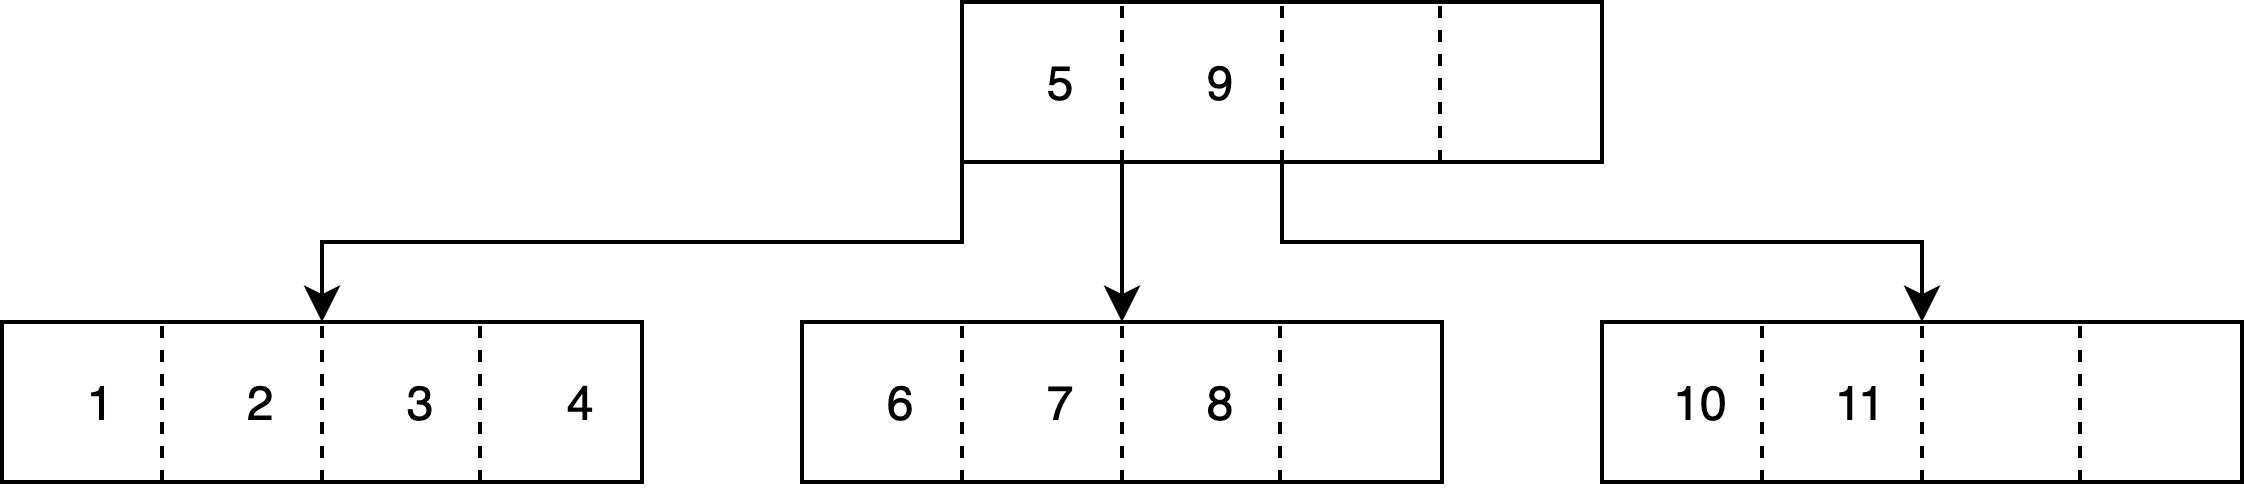
\includegraphics[align=c,width=10cm,keepaspectratio]{images/btree.png}
\end{frame}

\begin{frame}{Преимущества B дерева}
  Иерархия памяти:
  \begin{enumerate}
    \item чтение из кеша CPU \textapprox 10 нс
    \item чтение из памяти \textapprox 100 нс
    \item чтение с диска \textapprox 10 мс
  \end{enumerate}
  \vspace{2em}
  \begin{itemize}
    \item $10^8$ записей в БД
    \item строковый ключ 64 символа
    \item указатель на запись 8 байт
    \item 4 Кб узел дерева \rarr порядок дерева = 56
    \item высота дерева \rarr $log_{56} 10^8 \approx 5$
    \item высота двоичного дерева $\approx 27$
  \end{itemize}
\end{frame}

\begin{frame}{B+ дерево}
  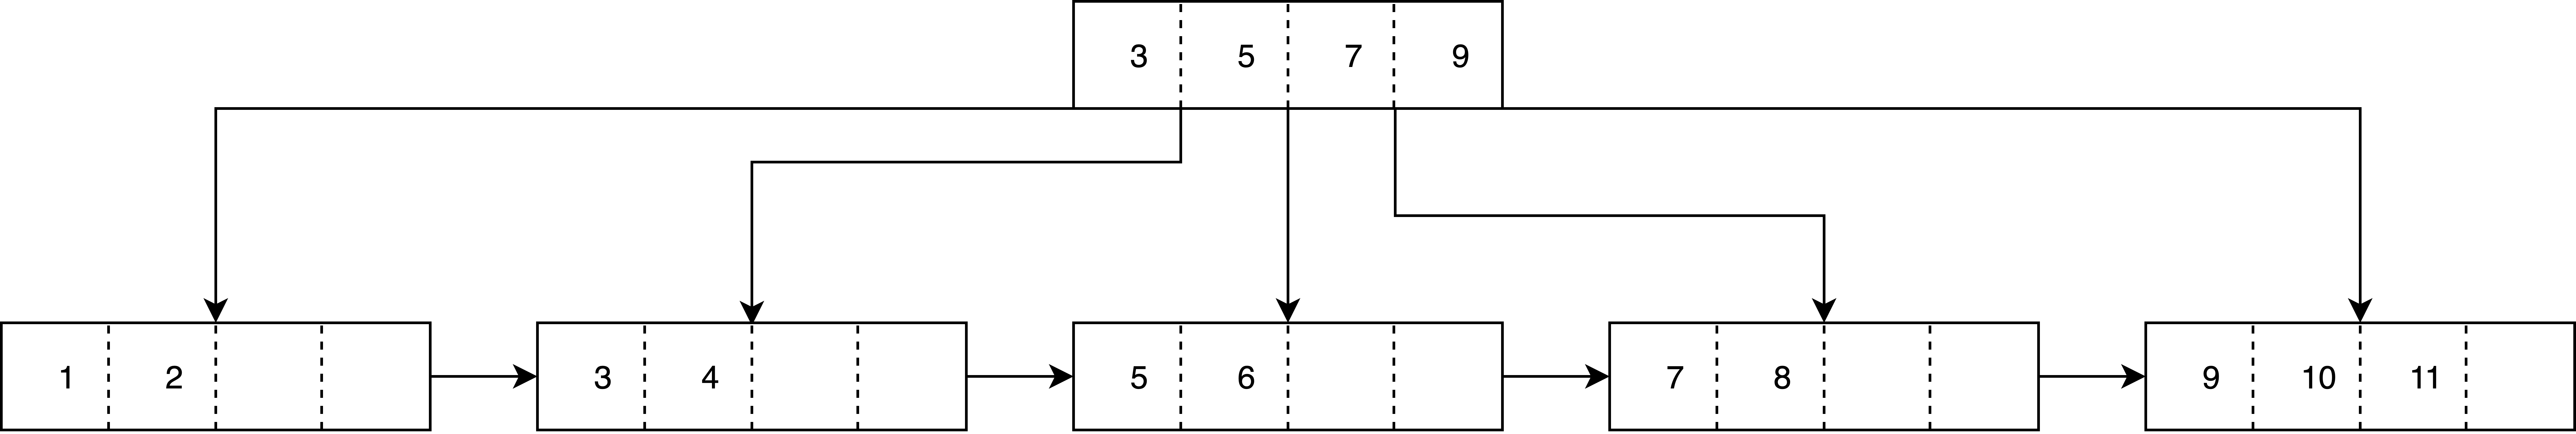
\includegraphics[align=c,width=11cm,keepaspectratio]{images/bptree.png}
\end{frame}

\begin{frame}{B+ дерево, вставка}
  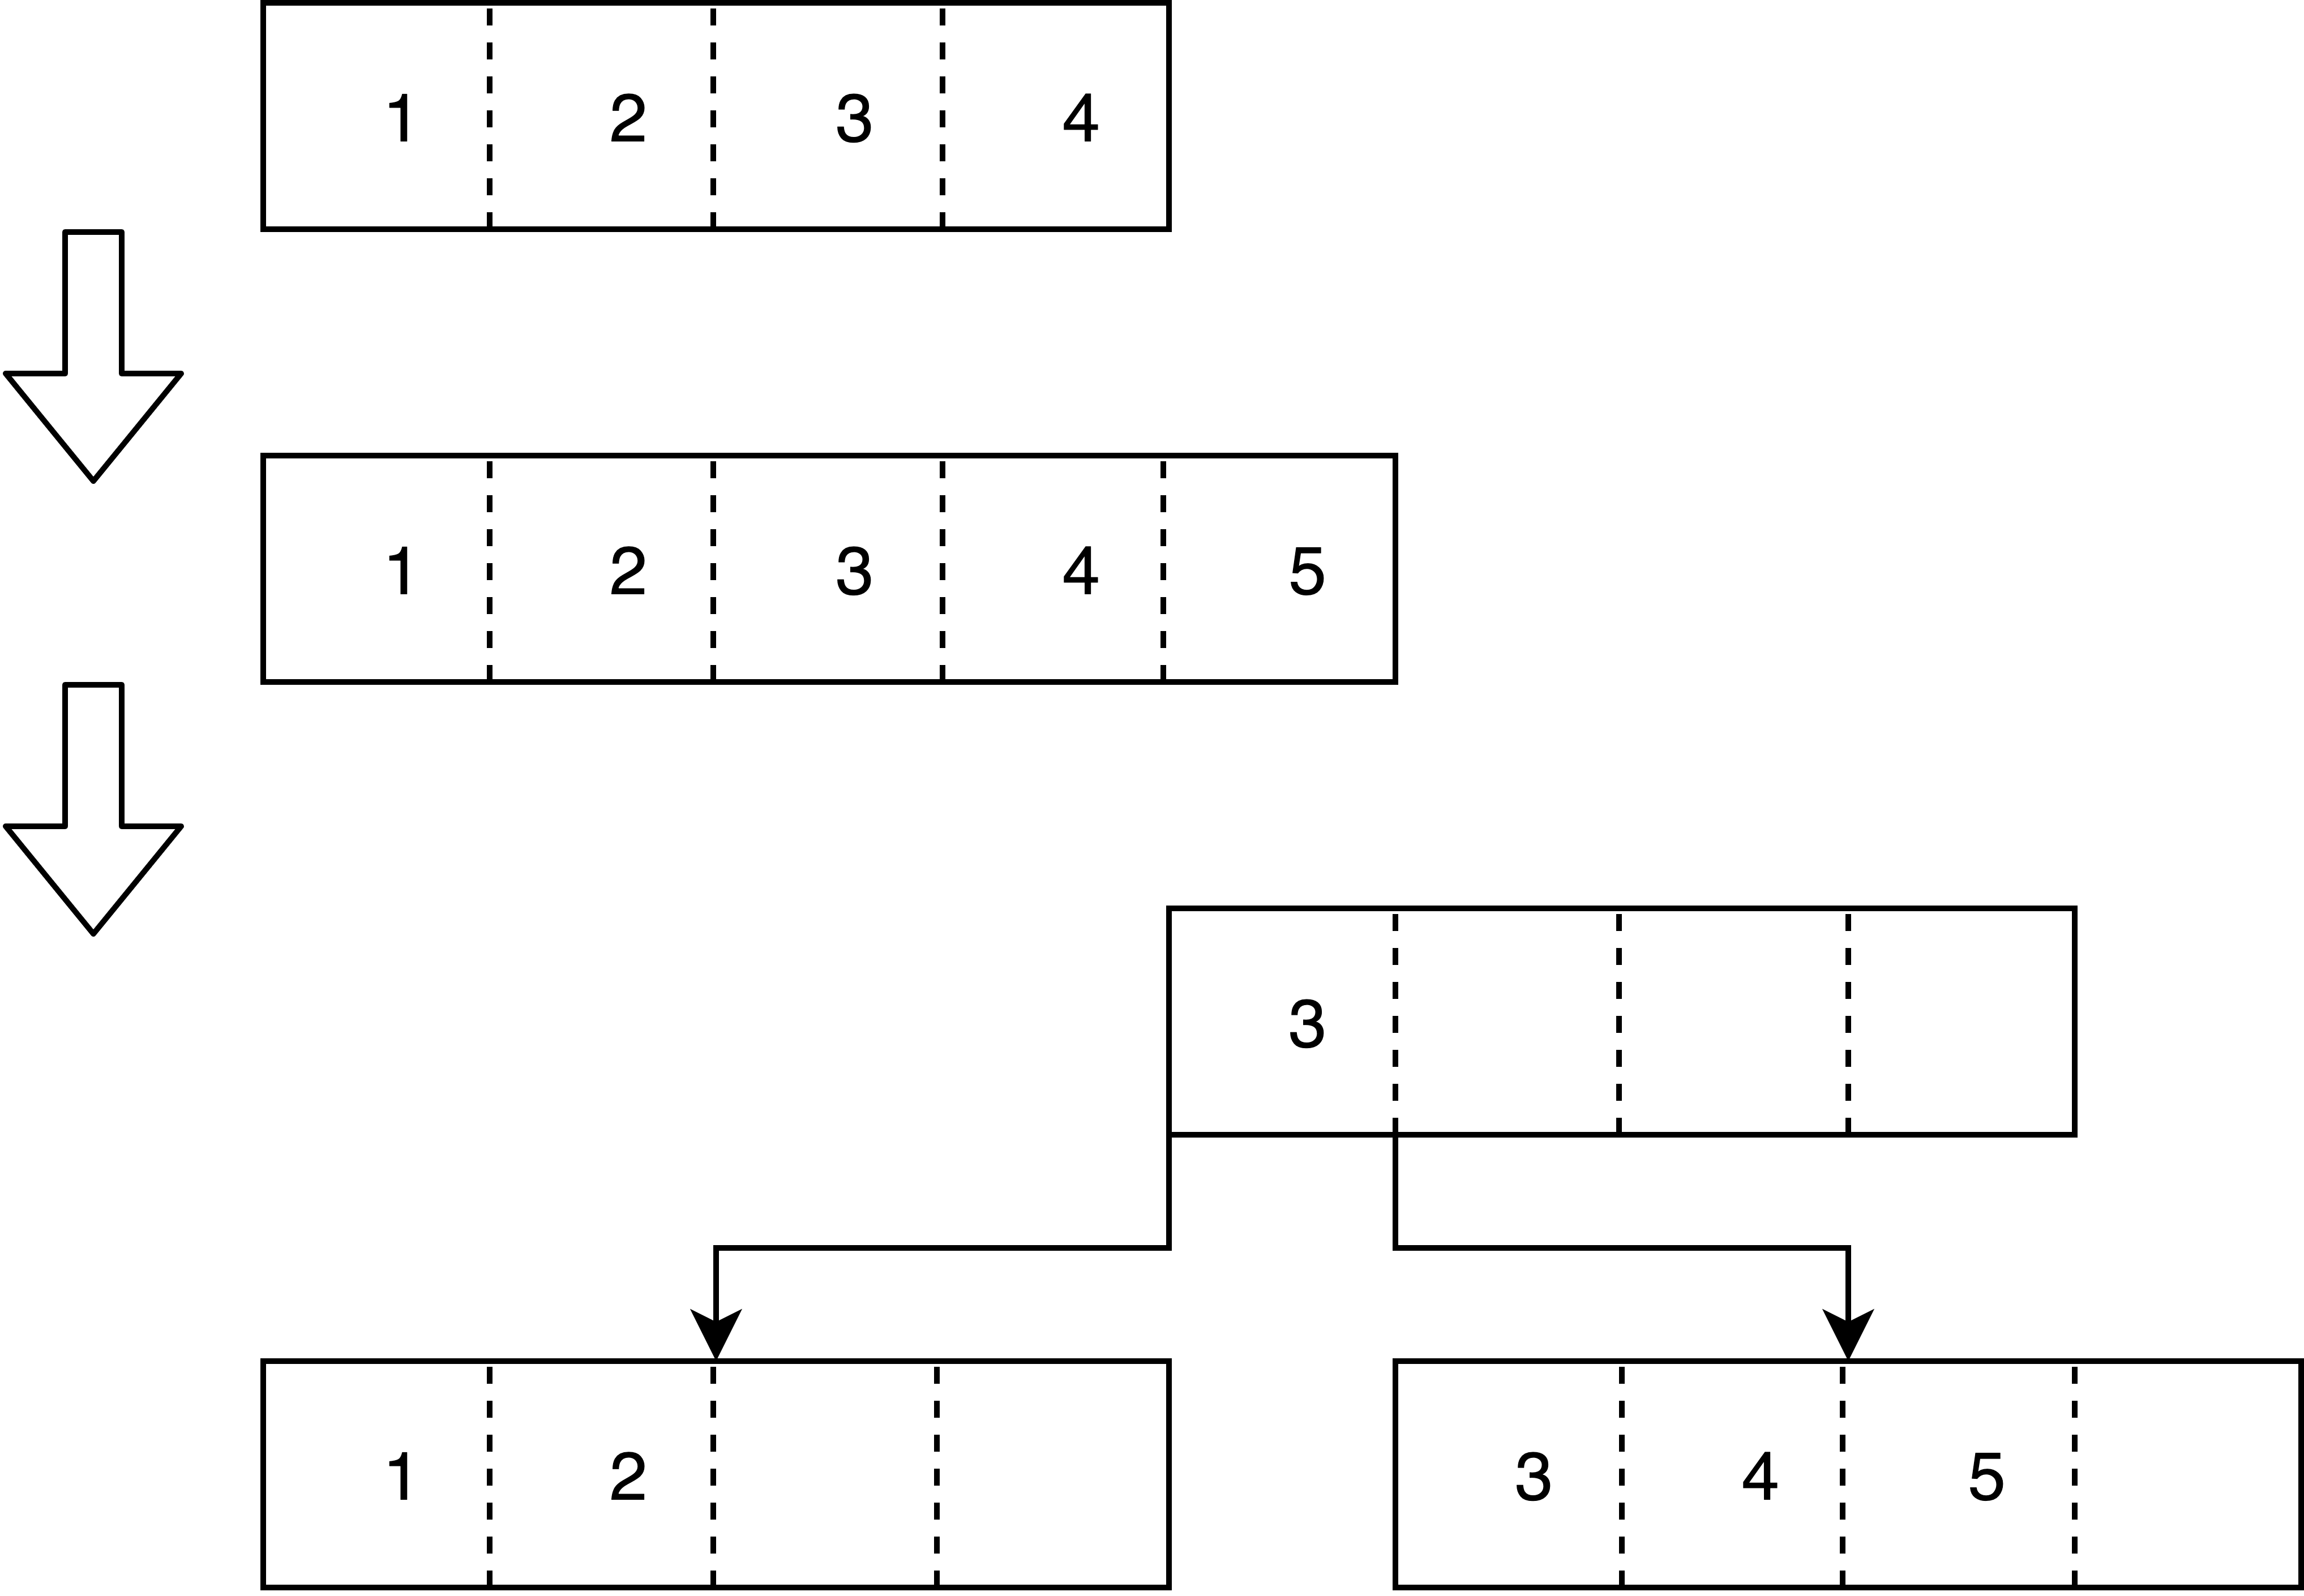
\includegraphics[align=c,width=8cm,keepaspectratio]{images/bptree_insert.png}
\end{frame}

\begin{frame}{B+ дерево, удаление}
  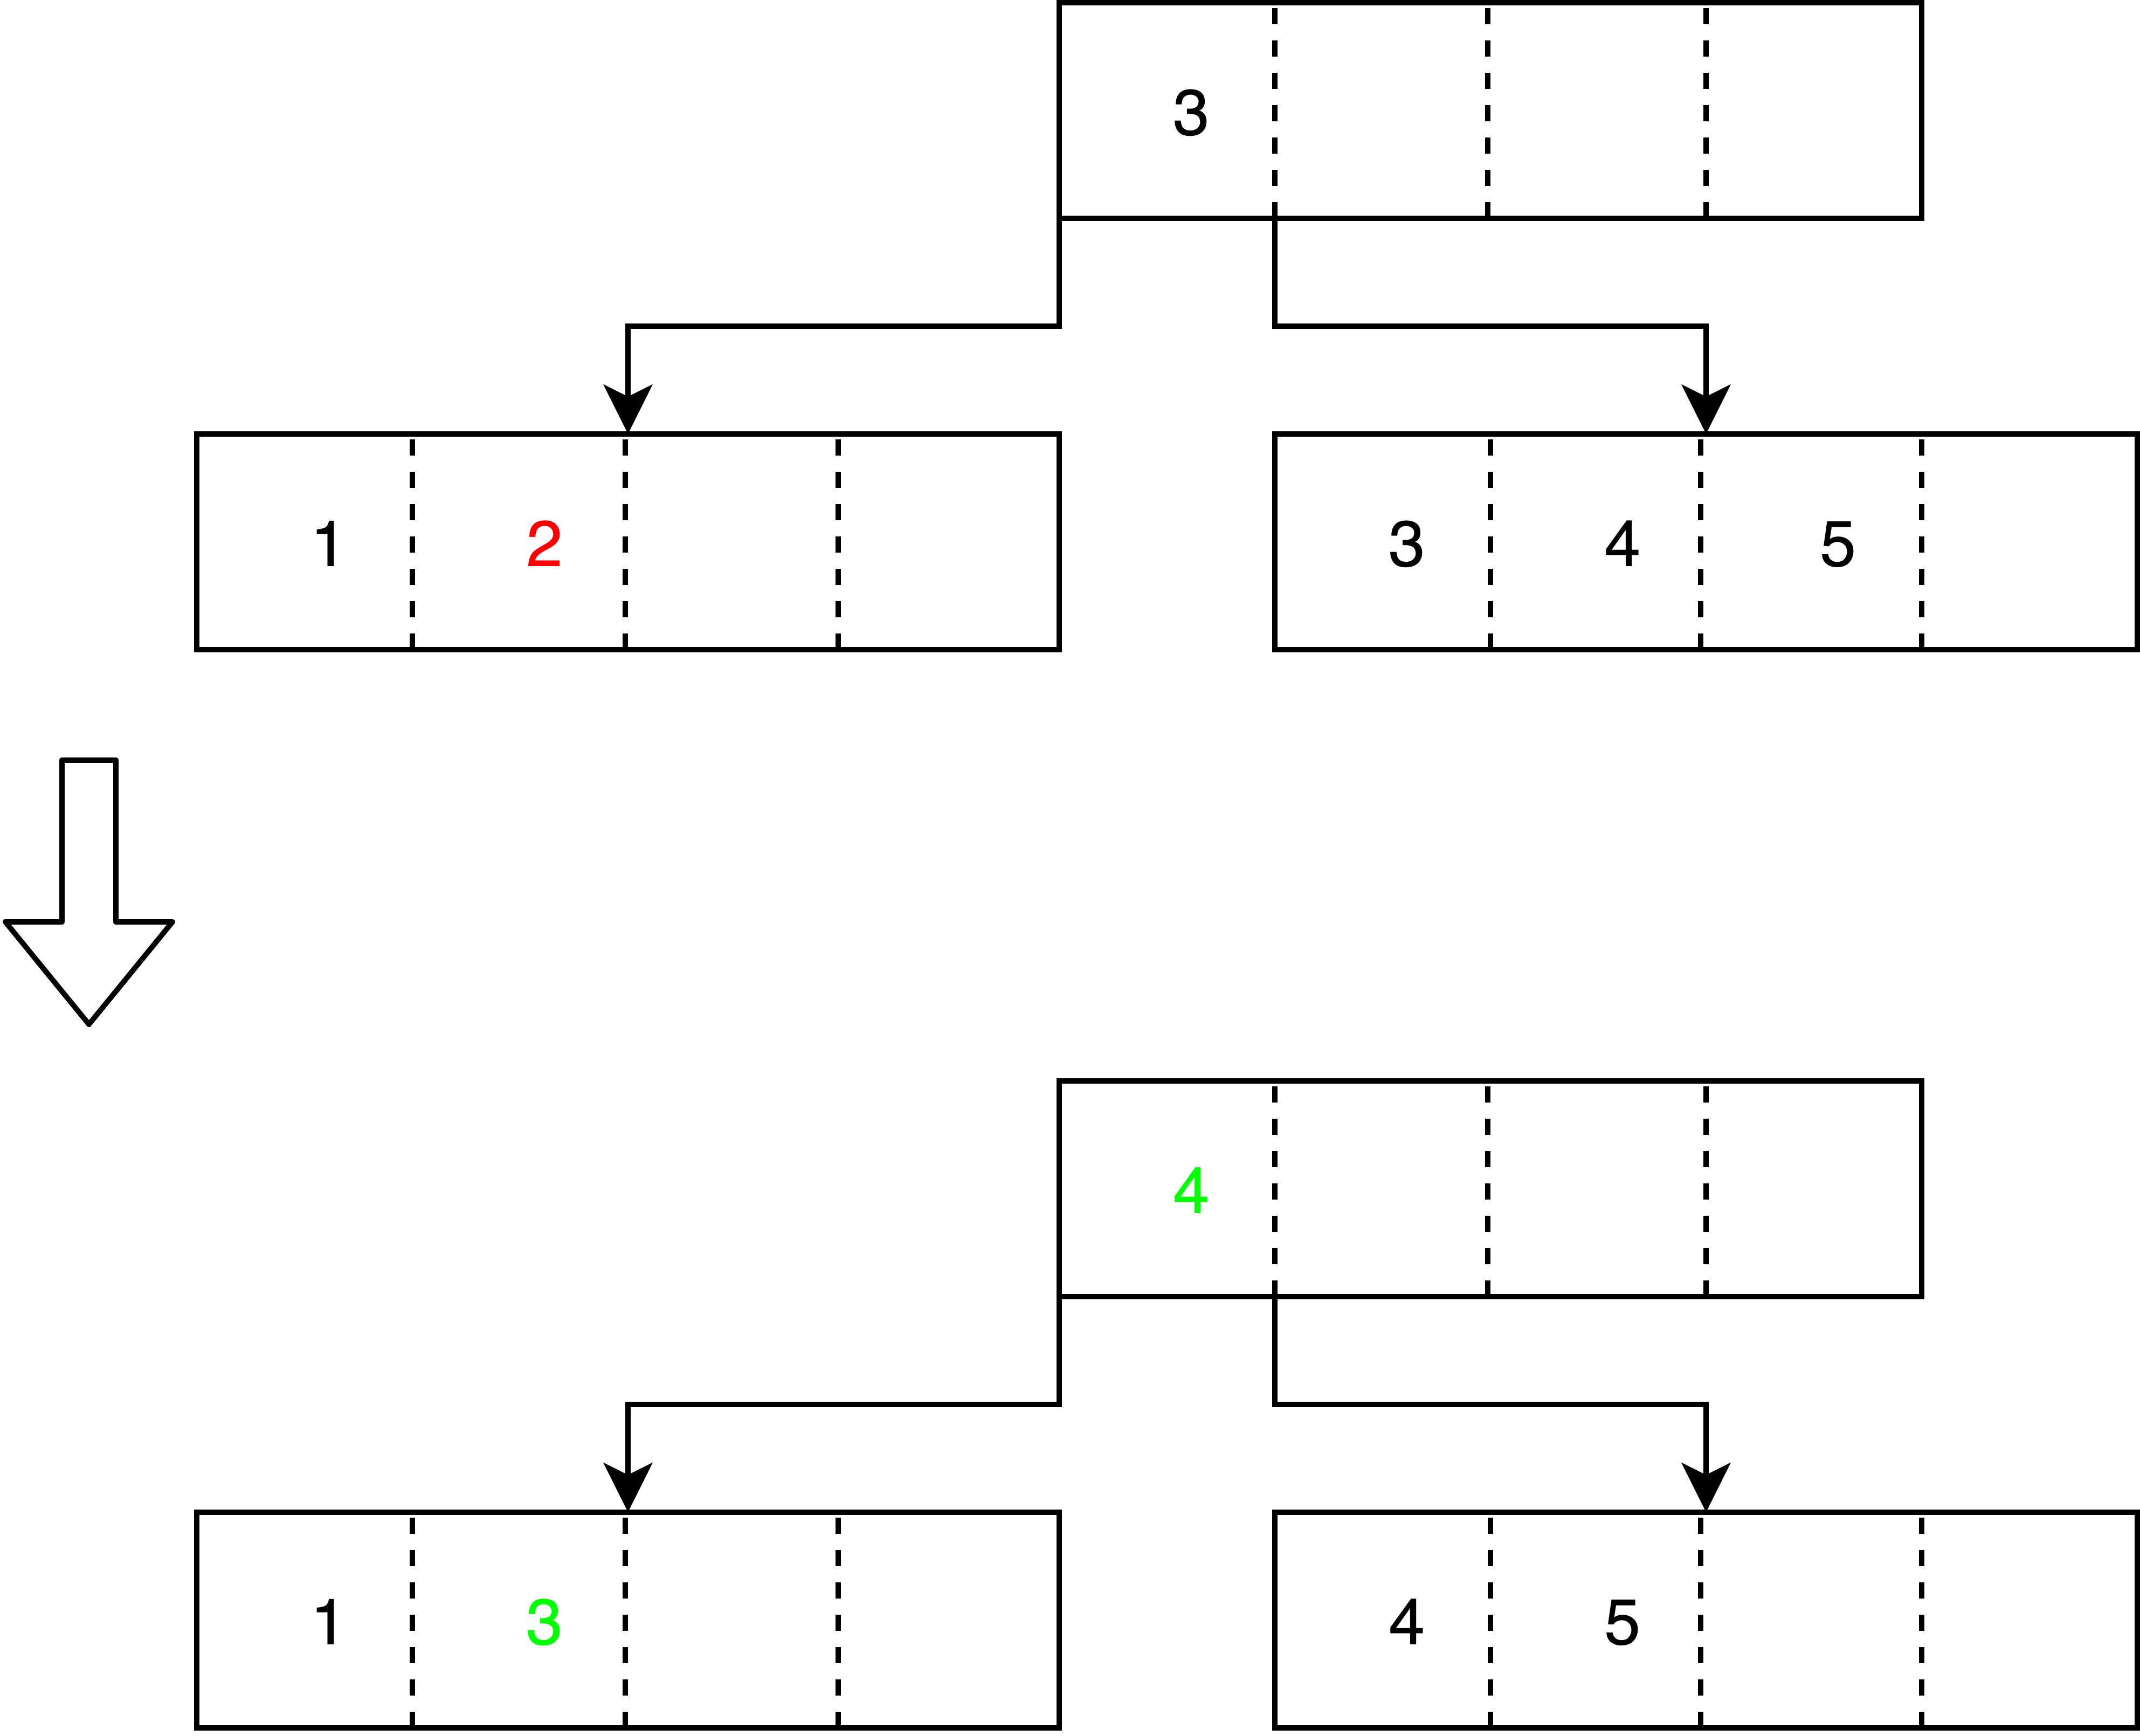
\includegraphics[align=c,width=8cm,keepaspectratio]{images/bptree_delete.png}
\end{frame}

\section{Краткое введение в динамический полиморфизм}

\begin{frame}[fragile]{Виртуальные методы}
  \begin{lstlisting}[basicstyle=\ttfamily\srcmediumsize]
    class Base
    {
      int m_x = 0;
    public:
      virtual std::ostream & print(std::ostream & strm) const
      { return strm << m_x; }

      virtual Base * clone() = 0;
    };

    class Derived : Base
    {
      double m_y = 0;
    public:
      std::ostream & print(std::ostream & strm) const override
      { return Base::print(strm) << m_y; }

      Base * clone() override
      { return new Derived; }
    };

    std::ostream & print(std::ostream & strm, const std::vector<Base *> & objs)
    {
      for (const auto p : objs) {
        p->print(strm);
      }
      return strm;
    }
  \end{lstlisting}
\end{frame}

\begin{frame}[fragile]{Виртуальный деструктор}
  \begin{lstlisting}
    struct Base
    {
      virtual ~Base() {}
    };

    struct Derived : Base
    {
      ~Derived();
    };

    int main()
    {
      Base * b = new Derived;
      delete b;
    }
  \end{lstlisting}
\end{frame}

\section{Некоторые аспекты обобщённых интерфейсов}

\begin{frame}[fragile]{Шаблонные аргументы}
  \begin{lstlisting}
    template <class T>
    class Queue
    {
    public:
        void push(?);
    };

    X get_x();

    void process(Queue<X> & queue, const X & x1, X & x2)
    {
        queue.push(x1);
        queue.push(x2);
        queue.push(get_x());
        queue.push(X{});
        queue.push(97);
    }
  \end{lstlisting}
\end{frame}

\begin{frame}[fragile]{Шаблонные аргументы, продолжение}
  \begin{lstlisting}
    template <class T>
    class Queue
    {
    public:
        void push(const T & x);
        void push(T && x);
        
        template <class P>
        void push(P && p);
    };
  \end{lstlisting}
\end{frame}

\begin{frame}[fragile]{Шаблонные аргументы, сложности}
  \begin{lstlisting}
    class Queue
    {
    public:
        template <class P>
        void push(const P & p);

        template <class P>
        void push(P && p); // lvalue or rvalue reference??
    };
  \end{lstlisting}
\end{frame}

\begin{frame}[fragile]{Вывод шаблонных параметров-типов}
  \begin{lstlisting}[basicstyle=\ttfamily\srcsize]
    #include <iostream>
    #include <string>

    template <class T>
    void pretty_print(T && t, const char * label)
    {
        std::cout << __PRETTY_FUNCTION__ << std::endl;
        std::cout << label << " : " << t << std::endl;
    }

    std::string get_str() { return "Hello!"; }

    struct X
    {
        double x = 111.01;

        void test_print() const
        { pretty_print(x, "x"); }
    };

    int main()
    {
        int a = 10;
        const int b = 5;
        std::string s1 = "First";
        const std::string s2 = "Second";

        pretty_print(a, "a");
        pretty_print(b, "b");
        pretty_print(s1, "s1");
        pretty_print(s2, "s2");
        pretty_print(get_str(), "get_str()");
        X x;
        x.test_print();
    }
  \end{lstlisting}
\end{frame}

\begin{frame}[fragile]{Вкратце о копировании и перемещении}
  \begin{lstlisting}
    X get_x();

    X x;
    auto x1 = x;
    auto x2 = get_x();
    auto x3 = std::move(x);
  \end{lstlisting}
\end{frame}

\begin{frame}[fragile]{Сохранение rvalue ссылки при передаче в другие методы}
  \begin{lstlisting}
    void push(std::vector<X> & v, X && x)
    {
        v.push_back(x); // copy
        v.push_back(std::move(x)); // move
    }
  \end{lstlisting}
\end{frame}

\begin{frame}[fragile]{Идеальная передача шаблонных ссылок}
  \begin{lstlisting}
    template <class T>
    void push(std::vector<X> & v, T && x)
    {
        v.emplace_back(std::forward<T>(x));
    }

    template <class... Args>
    void push(std::vector<X> & v, Args && ...args)
    {
        v.emplace_back(std::forward<Args>(args)...);
    }
  \end{lstlisting}
\end{frame}

\begin{frame}[fragile]{Передача нескольких групп параметров в одном variadic списке}
  \begin{lstlisting}
    template <class... Args>
    void insert(std::unordered_map<std::string, X> & data, const char * key, std::size_t key_len, Args &&... args)
    {
      data.emplace(
        std::piecewise_construct,
        std::forward_as_tuple(key, key_len),
        std::forward_as_tuple(args...));
    }
  \end{lstlisting}
\end{frame}

\end{document}
